\chapter{Introdução}

\citeonline{hustrulid2013open} fragmentam a evolução de uma mina em três fases distintas: (1) Planejamento, (2) Implementação e (3) Produção. A \autoref{seq_min} é uma linha do tempo mostrando a relação entre as diferentes fases e seus estágios. Na fase de planejamento os depósitos minerais são investigados no que diz respeito à sua atratividade econômica e exequibilidade técnica. A fase de planejamento culmina em um relatório de viabilidade, no qual é baseada a decisão de investir e dar continuidade ao empreendimento mineiro, iniciando a fase de implementação, período de maior fluxo de caixa, quando mina e usina de processamento são desenvolvidas. Finalmente a mina entra em operação, o minério é explotado e processado, e o produto vendido no mercado.     

\begin{figure}[!htb]
	\caption{\label{seq_min}Fases da mineração.}
	\begin{center}
		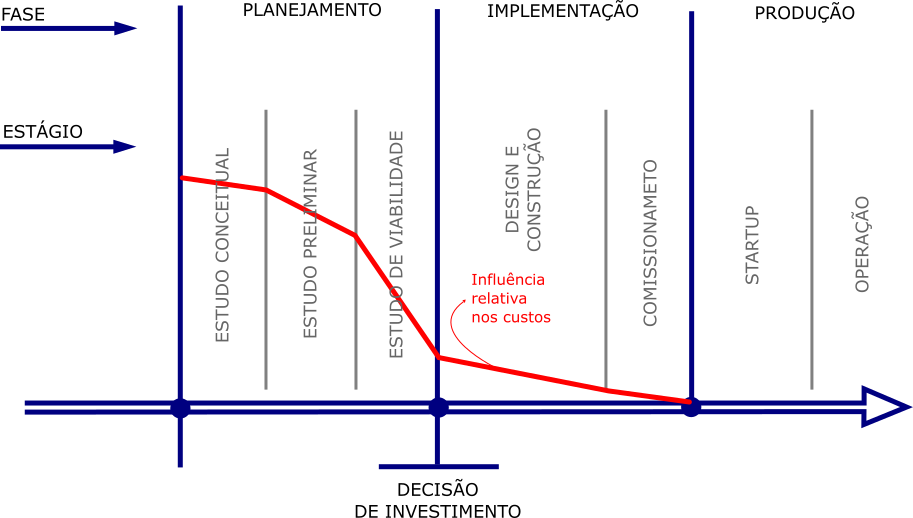
\includegraphics[width=0.6\textwidth]{introducao/min_fases}
	\end{center}
	\legend{Modificado de \citeonline{hustrulid2013open}}
\end{figure}

A avaliação das reservas é parte fundamental e alicerce do estudo de viabilidade, os teores e tonelagens são quantificados e modelos numéricos que caracterizam a geologia em subsuperfície criados com base nos dados de sondagem. A partir desses modelos, engenheiros e geólogos planejam e tomam as decisões econômicas e técnicas: Escolha do método de lavra, alternativas de processamento mineral, operações auxiliares, estimativas de custos operacionais, capital de investimento e projeção do lucro. Como resultado, uma estratégia que determina quanto material será removido ano a ano é traçada. O projeto determina os limites econômicos da mina e a sequência ótima de lavra bloco a bloco, baseado no modelo geoestatístico de blocos.

Na fase de planejamento é possível  minimizar o capital e custo operacional do projeto final e ao mesmo tempo maximizar a operabilidade e lucro. A influência relativa nos custos de cada fase é mostrado na linha vermelha da \autoref{seq_min} \cite{hustrulid2013open}. A principal causa de fracasso em empreendimentos mineiros é falta de conhecimento a respeito do corpo mineralizado. Isto posto, estimativas precisas e acuradas são importantes. Até mesmo um pequeno desvio entre produção planejada e real pode causar sérios prejuízos financeiros.
 
A avaliação dos recursos de uma mina é composta de duas etapas \cite{chiles2004modelling}: (1) delimitação das várias unidades geológicas, correspondentes às diferentes formações geológicas ou diferentes litologias; (2) estimativas e/ou simulação de teores em cada unidade modelada.

Desse modo, previamente à toda estimativa e/ou simulação de teores, há a necessidade de delimitar as unidades geológicas, implicando em decisão de estacionariedade e homogeneidade mineralógica em cada domínio modelado. Isto é, Os teores de cada domínio geológico pertencem a diferentes populações estatísticas e são caracterizados através de modelos de distribuição e semivariogramas específicos, resultando em estimativas e/ou simulações distintas para cada população \cite{mclennan}.

Modelos geológicos descrevem a extensão, forma e volume das diferentes unidades geológicas no espaço. Gerar modelos geológicos corretos é necessário para que estimativas mais precisas de volume/massa e teores sejam obtidas e problemas de diluição ocasionados pela falta de aderência do modelo de blocos às estruturas geológicas do depósito sejam reduzidos \cite{rasera2014estrati}.

Tradicionalmente os modelos geológicos são criados explicitamente, através de um processo de digitalização dos contatos geológicos. Polígonos são construídos manualmente em seções, por um geomodelador, honrando os dados amostrais, esses polígonos são conectados por linhas-guia e então interpolados por triangulação, gerando sólidos que representam as unidades geológicas. Esse processo apresenta alguns pontos críticos segundo \citeonline{cowan2003practical}:
\begin{itemize}
\item É demorado e requer um geomodelador experiente; 
\item É subjetivo, já que cada geomodelador interpretará, e produzirá um modelo diferente a partir do mesmo banco de dados, tornando replicação e auditoria externa do modelo tarefas árduas;
\item  É inflexível, pois atualizar o modelo à medida que novos dados são adquiridos é demorado e laborioso. 
\end{itemize}

Para muitas minas, apenas um único modelo geológico é mantido, dada a limitação de tempo imposta pelos métodos explícitos. Raramente há oportunidade de modelar interpretações alternativas e comparar estimativas de recursos baseadas em diferentes modelos. Não havendo assim, oportunidade de avaliar as incertezas inerentes ao modelamento geológico \cite{cowan2003practical}.

Ainda que \textit{softwares} modernos de mineração forneçam ferramentas computacionais para visualizar os dados de sondagem e agilizar o processo de digitalização manual, os métodos explícitos ainda sofrem com as desvantagens apresentadas. Por esse motivo, novas técnicas, conhecidas como modelagem implícita, vêm surgindo. São algoritmos que reduzem o nível de subjetividade, substituindo o processo de digitalização manual por alguma forma de procedimento automático \cite{maureira}.

As técnicas de modelagem geológica implícita se dividem em dois grandes grupos: 

O grupo das técnicas determinísticas. Métodos diretos e computacionalmente rápidos. Alguns métodos estabelecidos nessa categoria são a interpolação suavizada discreta \cite{mallet2002geomodeling}, o método dos campos potenciais \cite{chiles2004modelling,calcagno2008geological,renard2013modeling}, operacionalizado no \textit{software Isatis}\textsuperscript{\textregistered}, e a metodologia implementada no \textit{software} de modelagem geológica \textit{Leapfrog}\textsuperscript{\textregistered} \cite{cowan2002rapid,cowan2003practical}, amplamente utilizado pela indústria.

O outro grupo compreende as técnicas estocásticas de modelagem geológica. Métodos complexos que demandam grande esforço computacional. Entretanto, no lugar de um único modelo geológico, esses métodos geram diversas realizações equiprováveis da distribuição espacial das diferentes litologias, reproduzindo os atributos estatísticos das amostras. Assim, a partir da análise conjunta das realizações é possível avaliar a incerteza associada ao modelo geológico. 

São métodos consolidados: A simulação sequencial dos indicadores \cite{journel1983nonparametric}, simulação sequencial gaussiana truncada \cite{journel1984conditional}, simulação plurigaussiana \cite{galli1994pros}, métodos baseados em simulação objetos (\textit{object-based}) \cite{bridge1979simulation}, recentemente surgiram os métodos de modelagem de superfície (\textit{surface-based}) \cite{pyrcz2005stochastic}. Contudo, os algoritmos tradicionais de simulação, baseados em estatísticas de dois pontos, não são capazes de reproduzir estruturas geológicas que apresentam complexas interdependências, assim surgem os métodos baseados em geoestatística multiponto (MPS) \cite{guardiano1993multivariate}.

\citeonline{silvaanddeutschccgmodeling} apresentaram a modelagem geológica implícita com funções distância assinaladas para modelar múltiplos domínios geológicos simultaneamente. \citeonline{deutschcoal} o utilizou para modelar múltiplas camadas de carvão, e mostrou que o método é uma poderosa ferramenta de modelagem. \citeonline{wildedeutschcalibrate} e \citeonline{silvaanddeutschccgcorrecting} introduziram duas medidas heurísticas diferentes de avaliação de incertezas e \citeonline{silvaanddeutschccgcorrecting} uma ferramenta para corrigir as proporções globais dos diferentes domínios. E mostraram, novamente, a competência do método. \citeonline{maureira} revisitou o método com a finalidade de construir, a partir dos dados amostrais, imagens de treinamento (\textit{data-driven training images}) que forneçam as estatísticas de múltiplos pontos (MPS) para a simulação de litologias. 

A modelagem geológica implícita com funções distância assinaladas é uma técnica determinística, baseada na interpolação de uma função distância em um \textit{grid}. Funções de distância assinaladas medem o grau de separação entre as diferentes litologias, e dependem da orientação, forma e extensão dos corpos geológicos. Distâncias positivas indicam o exterior do domínio enquanto distâncias negativas indicam o interior do domínio. As distâncias assinaladas são calculadas para cada ponto amostral e para cada litologia, e interpoladas para os locais não amostrados. Um modelo geológico é criado a partir dos valores estimados para as distâncias assinaladas. O método é computacionalmente eficiente, direto e não depende de funções matemáticas complicadas. Ainda assim, consegue reproduzir de maneira satisfatória estruturas geológicas de grande escala nos modelos numéricos \cite{maureira}.

Essa dissertação é uma extensão do trabalho de \citeonline{deutschcoal} e \citeonline{maureira}. Um \textit{plug-in} implementando o método no \textit{software SGeMS} foi desenvolvido e apresentado. A aplicabilidade do método mais uma vez foi posta à prova em um estudo de caso conduzido em um banco de dados real. E suas principais características, vantagens e limitações discutidas.

\section{Meta}

Essa dissertação de mestrado tem como meta investigar a aplicabilidade da modelagem geológica implícita com funções distância assinaladas como substituto ou método auxiliar à metodologia explícita de modelagem geológica, amplamente adotada pela indústria. Conhecidas as limitações e desvantagens da última e simplicidade e rapidez da primeira.

\section{Objetivos específicos}

A fim de atingir a meta proposta os seguintes objetivos foram delineados:
\begin{enumerate}
\item Operacionalizar o método no \textit{software} geoestatístico de código aberto \textit{SGeMS}, desenvolvendo um \textit{plug-in} funcional em \textit{python};
\item Conduzir um estudo de caso em um banco de dados real e verificar a qualidade do modelo gerado pela metodologia proposta, comparando-o a um modelo de referência.
\end{enumerate}

\section{Metodologia}

A partir de um banco de dados categóricos o valor da função distância assinalada é calculado para cada litologia em cada ponto amostral. As distâncias calculadas são então variografadas e interpoladas, por krigagem ordinária, para todo o \textit{grid}. Assim, o valor da função distância assinalada é conhecido em todos os nós e para cada litologia. Um modelo geológico pode ser criado diretamente a partir do valor estimado para as distâncias. Ou então, modelos de probabilidade podem ser criados a partir das distâncias. E então, um modelo geológico, que tem as proporções corrigidas para corresponder a uma proporção alvo, criado a partir dos modelos de probabilidade. A \autoref{chart} ilustra o fluxograma do processo. 

\begin{figure}[!htb]
	\caption{\label{chart}Fluxograma ilustrando a metodologia passo a passo.}
	\begin{center}
		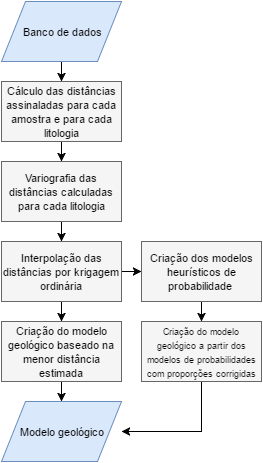
\includegraphics[width=0.4\textwidth]{introducao/chart1}
	\end{center}
	%\legend{Fonte: Modificado de \citeonline{hustrulid2013open}}
\end{figure}

O modelo criado implicitamente com a metodologia proposta foi comparado com um modelo criado explicitamente, a partir do mesmo banco de dados. Assim, foi possível checar se o algoritmo reproduziu satisfatoriamente as estruturas geológicas interpretadas pelo geomodelador.

\section{Estrutura da dissertação}

O capítulo 2 Revisa os conceitos de funções implícitas, estacionariedade e os principais métodos determinísticos de modelagem implícita baseados em funções implícitas: método dos campos potenciais, implementado no \textit{software Isatis}\textsuperscript{\textregistered}, e o método implementado no  \textit{software Leapfrog}\textsuperscript{\textregistered}.

O capítulo 3 apresenta o arcabouço teórico da modelagem geológica implícita com funções distância assinaladas, o \textit{plug-in} desenvolvido para o  \textit{software SGeMS} e os resultados da validação do algoritmo proposto tendo como referência resultados análogos da rotina \textit{DFMod} da biblioteca de algoritmos geoestatísticos \textit{GSLib}.

O capítulo 4 discute os resultados do estudo de caso conduzido em um banco de dados real, proveniente de um depósito de ouro. Avalia a aplicabilidade do método como substituto ou método auxiliar à metodologia tradicional (explicita) de modelagem geológica, comparando o modelo gerado a partir da metodologia proposta a um modelo de referência, criado explicitamente por um geomodelador. 

O capítulo 5 encerra a dissertação apresentando as conclusões do trabalho  e sugere trabalhos futuros relacionados ao tópico. 

